
%(BEGIN_QUESTION)
% Copyright 2003, Tony R. Kuphaldt, released under the Creative Commons Attribution License (v 1.0)
% This means you may do almost anything with this work of mine, so long as you give me proper credit

Complete the following ladder logic diagram so that an OR gate function is formed: the indicator lamp energizes if either switch A {\it or} switch B is actuated.

$$\includegraphics[width=15.5cm]{i02314x01.eps}$$

\vskip 20pt

Next, complete the following ladder logic diagram so that an AND gate function is formed: the indicator lamp energizes if both switch A {\it and} switch B are actuated.

$$\includegraphics[width=15.5cm]{i02314x01.eps}$$

\vskip 20pt

Finally, write the proper Boolean expression next to each lamp, describing its state in terms of A and B.

\underbar{file i02314}
%(END_QUESTION)





%(BEGIN_ANSWER)

$$\includegraphics[width=15.5cm]{i02314x02.eps}$$

$$\includegraphics[width=15.5cm]{i02314x03.eps}$$

%(END_ANSWER)





%(BEGIN_NOTES)

Discuss with students the fact that relay coils and contacts need not be located near each other in ladder diagrams.  While this may be confusing at times, it is a very flexible feature of ladder logic notation, because it gives the author the freedom to locate relay contacts where it makes the most visual sense in the ``output'' rung of the diagram, without having to coordinate locations of coil and contact as is generally necessary in traditional schematic diagrams.  Instead, relay contacts are associated with their respective coils {\it by label}, not by proximity on the diagram.

%INDEX% Relay, diagram: ladder logic

%(END_NOTES)


